\chapter{Implementation and Results}
In this section we cover the implementation of the project and the results.
As outlined in the Objectives section we can divide the tasks into three main
parts: generation, transmission, and reception. 
In this project we looked at using a FPGA board for the generation and
reception of the PRBS data.  Hence the overall design is of a board in a
loopback configuration as shown in Figure~\ref{fig:loopback}.

\begin{figure}[ht]
    \centering
    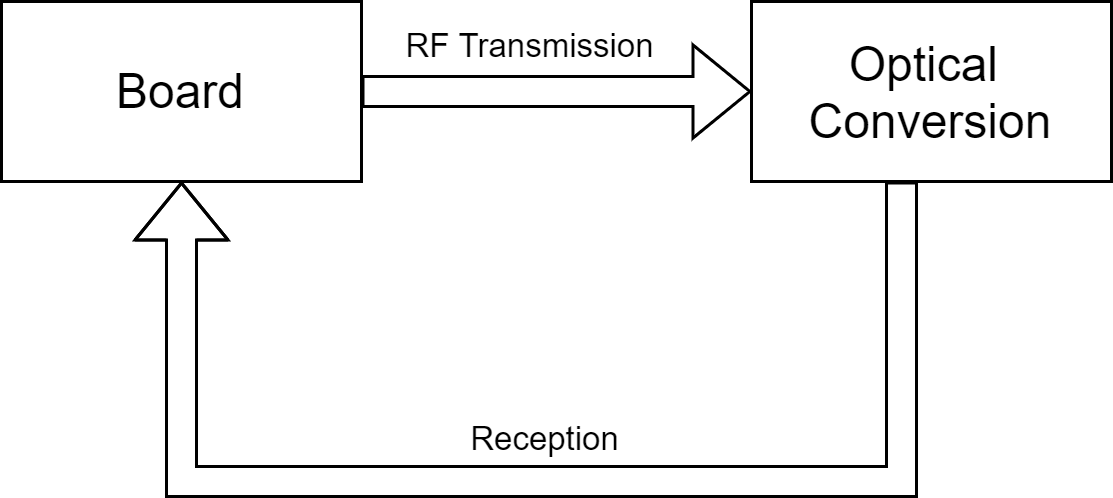
\includegraphics[width=0.6\linewidth]{img/loopback.png}
    \caption{Loopback Configuration}%
    \label{fig:loopback}
\end{figure}

\section{Generation and Reception}%
\label{sec:generation_and_reception}


\subsection{Hardware}%
\label{sub:hardware}
To generate and receive PRBS data the VCU118 board was used. The transmission
and reception of the data was handled by the onboard high-speed parallel to serial
GTY transceivers in conjuction with a Si5345 external clock (as the board is
not able to generate an internal clock to the needed precision).  The
full details of the setup can be found in the appendix.

\begin{figure}[ht]
    \centering
    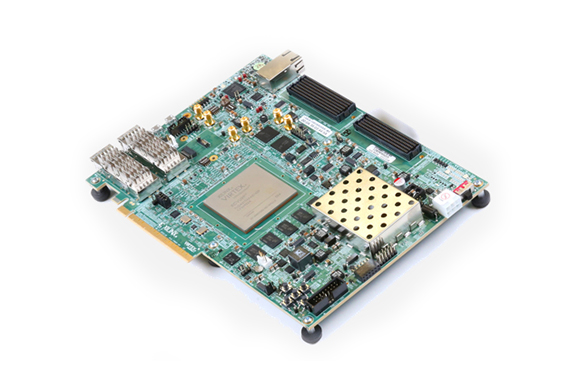
\includegraphics[width=0.4\linewidth]{img/board.jpg}
    \caption{VCU118 Board}%
    \label{fig:board}
\end{figure}

\begin{figure}[ht]
    \centering
    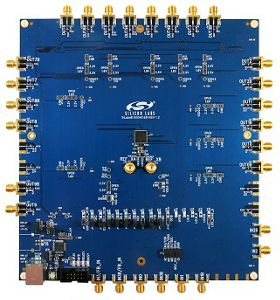
\includegraphics[width=0.4\linewidth]{img/clock.jpg}
    \caption{Si5345 Clock}%
    \label{fig:clock}
\end{figure}

\subsection{PRBS Generation}%
\label{sub:prbs_generation}

We looked to modify the functionality of a basic implementation of the
transceiver. In the basic implementation a PRBS generator is is fed to the
transceiver channel, through a wrapper. 
\TODO{image of prbsgen wrapped and passed to transceiver}

The PRBS module was unchanged from the default with the exception of reducing
the length of the PRBS sequence from PRBS31 (2.1 billion bits) to PRBS7 (511
bits) for ease of checking.
There were two variations of the PRBS generation module that were developed.

\subsubsection{Burst Mode over Single Channel}%
\label{ssub:burst_mode_over_single_channel}
Here we modified the PRBS generation module further and set it to output zeros
if the enable command was not asserted.  In combination we placed a 2 bit register inside
the wrapper, which on overflow toggles the enable flag. This has the effect of
causing the PRBS module to output a sequence interspersed with zeros.

\TODO{burst mode modification}

\subsubsection{Switching Between Two Channels}%
\label{ssub:switching_between_two_channels}
The main modification was to change the PRBS wrapper to feed the two different
outputs. The PRBS generator module was unchanged. Using a 2 bit register which
on oveflow alternated between which of the outputs the PRBS data was sent to, with
the other output being sent zeros. This had the overall effect of having the
whole sequence be sent over two different channels.

\TODO{two channel switch (showing module with two outputs)}


\subsection{PRBS Checking}%
\label{sub:prbs_checking}
In normal operation the transceiver would parallise the serial data, and then
pass the data to the PRBS checking module.  
\TODO{image of transceiver -> prbs module}

\subsubsection{Two Channel Checking}%
\label{ssub:two_channel_checking}
In the case where two transmitters were muxed together and were sent to a
single receiver, it should not have been necessary to change the behaviour of
the PRBS checking module.
However we were unable to check this as the lab was closed.

\subsubsection{Burst Mode Checking}%
\label{ssub:burst_mode_checking}
For burst mode checking there are some issues as there are periods when the
incoming bitstream is all zeros. The PRBS checker module takes the incoming
data as a seed to calculate the next expected sequence. If zeros are provided
then this interferes with the module (as the next expected word will be calculated
based on zeros). To compensate for this we added a register to the wrapper that
would not pass zeros to the checker module. In a basic simulation of PRBS generation
to PRBS checker this worked correctly, but when passed to through the
transceiver, the checker module would throw errors.  We were not able to determine why.

\subsubsection{Source Synchronous Reception}%
\label{ssub:source_synchronous_reception}
The final step would have been to run the reciever source synchronously. The
transceiver did not allow much flexibilty here. We attemped to do this was by
disabling the CDR and using the same clock to drive the reciever and
transmitter. However the link here was not stable, and we were unable to get
phase readouts that may have allowed us to modify the phase of the incoming
clock. Overall this was unsuccessful.


\section{Optical Transmission}%
\label{optical_transmission}
This part of the project was not completed as the labs were closed before we
were able to test it. However some hardware was prepared, and is described in
the following sections.
\subsection{SOA Board}%
\label{sub:soa_board}

\subsection{Heatsink and Mount}%
\label{sub:heatsink_and_mount}





